\documentclass{article}
\usepackage[utf8]{inputenc}
\usepackage[margin = 0.8in]{geometry}
\usepackage{graphicx}
\usepackage{amsmath, amssymb}
\usepackage{subcaption}
\usepackage{multirow}
\usepackage{mathtools}
\usepackage{float}
\usepackage{enumitem}

\DeclareMathOperator*{\wrote}{Wrote}
\DeclareMathOperator*{\copyof}{CopyOf}
\DeclareMathOperator*{\owns2}{Owns}
\DeclareMathOperator*{\sings}{Sings}


\title{CS534 - HW 1}
\author{Keith Chester}
\date{Due date: June 12 2022}

\begin{document}
\maketitle

\section*{Problem 1}

In problem 1, we are tasked with creating a recursive and linear time agent for following propositonal logic statements. The work associated with this problem can be found in \textit{problem1.py}.

\section*{Problem 2}

In this problem we are exploring a first-order logical knowledge base and writing out logical expressions utilizing it. The knowledge base is represented as:

\begin{itemize}
    \item $\copyof(d, a)$ - Predicate - Disk $d$ is a copy of album $a$
    \item $\owns2(p, d)$ - Predicate - Person $p$ owns disk $d$
    \item $\sings(p, s, a)$ - Predicate - Album $a$ inludes a recording of song $s$ sung by person $p$
    \item $\wrote(p, s)$ - Person $p$ wrote song $s$

\end{itemize}

We are also injecting the following constants:
\begin{itemize}
    \item $McCartney$ - a person
    \item $Gershwin$ - a person
    \item $BHoliday$ - a person
    \item $Joe$ - a person
    \item $EleanorRigby$ - a song
    \item $TheManILove$ - a song
    \item $Revolver$ - an album
\end{itemize}

\noindent Within this, we express the following statements using first-order logic:

\begin{enumerate}[label=(\alph*)]
    \item $\wrote(Gershwin, TheManILove)$ %a
    \item $\neg \wrote(Gershwin, EleanorRigby)$ %b
    \item $\wrote(Gershwin, TheManILove) \lor \wrote(McCartney, TheManILove)$ %c
    \item $\exists s \wrote(Joe, s)$ %d
    \item $\exists d \owns2(Joe, CopyOf(d, Revolver))$
    \item $\forall s \sings(McCartney, s, Revolver) \Rightarrow \wrote(McCartney, s)$ %f
    \item $\forall s \sings(p, s, Revolver) \neg \wrote(Gershwin, s)$ %g
    \item $\forall s \wrote(Gershwin, s) \Rightarrow \sings(p, s, a)$ %h
    \item $\exists a \forall s \sings(p, s, a) \wrote(Joe, s)$ %i
    \item $\exists d, a \owns2(Joe, \copyof(d, a)) \land \sings(BHoliday, s, a)$ %j
    \item $\exists d_i \copyof(d_i, a) \forall a \sings(McCartney, a, s) \land \forall  \owns2(Joe, d)$ %k
    \item $\exists d \copyof(d, a) \forall a \sings(BHoliday, s, a) \land \owns2(Joe, d)$ %l
\end{enumerate}

\section*{Problem 3}

In this queston, we are looking at the following table of three binary input atributes, and a singular binary output:

\begin{center}
    \begin{tabular}{ c r r r r }
        Example & $A_1$ & $A_2$ & $A_3$ & Output $y$\\ 
        $x_1$ & $1$ & $0$ & $0$ & $0$\\
        $x_2$ & $1$ & $0$ & $1$ & $0$\\
        $x_3$ & $0$ & $1$ & $0$ & $0$\\
        $x_4$ & $1$ & $1$ & $1$ & $1$\\
        $x_5$ & $1$ & $1$ & $0$ & $1$\\
    \end{tabular}
\end{center}

\subsection*{a.}

Using the Gini Index, we aim to create a decision tree for this data. For Gini Index, we are looking at the probability distribution of a particular variable being wrong when randomly chosen. From this we can begin to branch our tree into a set of decisions that lead us to a particular preditctive result.

\begin{equation}
    Gini = 1-\sum^{n}_{i=1} p_i^2
\end{equation}

\noindent ...where $p_i$ is the probability of a given object being classified into a particular class.

So, calculating the Gini index for our given data:

\noindent For $A_1$, we are look at the indexes of positive and negative outputs:

\begin{equation}
    {A_1=1,y=1} \rightarrow \frac{2}{4} = 0.5
\end{equation}
\begin{equation}
    {A_1=1,y=0} \rightarrow \frac{2}{4} = 0.5
\end{equation}
\noindent ...for the Gini calculation of:
\begin{equation}
    1-(0.5^2 + 0.5^2) = 0.5
\end{equation}
\begin{equation}
    {A_1=0,y=1} \rightarrow \frac{0}{1} = 0
\end{equation}
\begin{equation}
    {A_1=0,y=0} \rightarrow \frac{1}{1} = 1
\end{equation}
\noindent ...for the Gini calculation of:
\begin{equation}
    1-(0^2 + 1^2) = 0
\end{equation}
\noindent and the weighted sum of these Gini indexes to create the Gini index for $A_1$:
\begin{equation}
    \sum p_i * g_i = (\frac{4}{5}*0.5 + \frac{1}{5}*0) = 0.4
\end{equation}

\noindent Now we continue this for $A_2$:

\begin{equation}
    {A_2=1,y=1} \rightarrow \frac{2}{3} = 0.67
\end{equation}
\begin{equation}
    {A_2=1,y=0} \rightarrow \frac{1}{3} = 0.33
\end{equation}
\noindent ...for the Gini calculation of:
\begin{equation}
    1-(0.67^2 + 0.33^2) = 0.44
\end{equation}
\begin{equation}
    {A_2=0,y=1} \rightarrow \frac{0}{2} = 0
\end{equation}
\begin{equation}
    {A_2=0,y=0} \rightarrow \frac{2}{2} = 1
\end{equation}
\noindent ...for the Gini calculation of:
\begin{equation}
    1-(0^2 + 1^2) = 0
\end{equation}
\noindent and the weighted sum of these Gini indexes to create the Gini index for $A_2$:
\begin{equation}
    \sum p_i * g_i = (\frac{3}{5}*0.44 + \frac{2}{5}*0) = 0.27
\end{equation}

\noindent ...and finally, following the process for $A_3$:

\begin{equation}
    {A_3=1,y=1} \rightarrow \frac{1}{2} = 0.5
\end{equation}
\begin{equation}
    {A_3=1,y=0} \rightarrow \frac{1}{2} = 0.5
\end{equation}
\noindent ...for the Gini calculation of:
\begin{equation}
    1-(0.5^2 + 0.5^2) = 0.5
\end{equation}
\begin{equation}
    {A_3=0,y=1} \rightarrow \frac{1}{3} = 0.33
\end{equation}
\begin{equation}
    {A_3=0,y=0} \rightarrow \frac{2}{3} = 0.67
\end{equation}
\noindent ...for the Gini calculation of:
\begin{equation}
    1-(0.33^2 + 0.67^2) = 0.44
\end{equation}
\noindent and the weighted sum of these Gini indexes to create the Gini index for $A_3$:
\begin{equation}
    \sum p_i * g_i = (\frac{2}{5}*0.5 + \frac{3}{5}*0.44) = 0.27
\end{equation}

\noindent So the Gini indexes for each input is 

\begin{center}
    \begin{tabular}{l r}
        Input & Gini index \\
        $A_1$ & 0.4 \\
        $A_2$ & 0.27 \\
        $A_3$ & 0.27
    \end{tabular}
\end{center}

Both $A_3$ and $A_2$ have the same Gini index, thus either can be utilized as the root node of our decision tree. For our purposes, we will choose $A_3$. From this we repeat the computations above for the positive and negative branches of our $A_3$ input.

\noindent \textbf{Positive $A_3$:}

\begin{center}
    \begin{tabular}{ c r r r r }
        Example & $A_1$ & $A_2$ & $A_3$ & Output $y$\\ 
        $x_2$ & $1$ & $0$ & $1$ & $0$\\
        $x_4$ & $1$ & $1$ & $1$ & $1$\\
    \end{tabular}
\end{center}

\noindent Gini Index of $A_1=1$ when $A_3=1$:

\begin{equation}
    {A_1=1,y=1} \rightarrow \frac{1}{2} = 0.5
\end{equation}
\begin{equation}
    {A_1=1,y=0} \rightarrow \frac{1}{2} = 0.5
\end{equation}
\begin{equation}
    1 - (0.5^2 + 0.5^2) = 0.5
\end{equation}

\noindent Gini Index of $A_1=0$ when $A_3=1$ is not applicable, as there is no examples anymore of $A_1$ = 0. Thus our weighted Gini Index is still $0.5$.

\noindent Gini Index of $A_2=1$ when $A_3=1$:

\begin{equation}
    {A_2=1,y=1} \rightarrow \frac{1}{1} = 1.0
\end{equation}
\begin{equation}
    {A_2=1,y=0} \rightarrow \frac{0}{1} = 0.0
\end{equation}
\begin{equation}
    1 - (1.0^2 + 0.0^2) = 0.0
\end{equation}

\noindent Ginin  Index of $A_2=0$ when $A_3=1$:

\begin{equation}
    {A_2=1,y=1} \rightarrow \frac{0}{1} = 0.0
\end{equation}
\begin{equation}
    {A_2=1,y=0} \rightarrow \frac{1}{1} = 1.0
\end{equation}
\begin{equation}
    1 - (0^2 + 1.0^2) = 0.0
\end{equation}

\noindent ...for a Gini index, when weighted, to still be $0.0$ for $A_2$.

\begin{center}
    \begin{tabular}{l r}
        Input & Gini index \\
        $A_1$ & 0.5 \\
        $A_2$ & 0.0 \\
    \end{tabular}
\end{center}

\noindent ...so we see that we want to use $A_2$ for the next split as it has the lowest Gini index, and completes this branch of the tree as we have a perfect split.

\noindent \textbf{Negative $A_3$:}

\begin{center}
    \begin{tabular}{ c r r r r }
        Example & $A_1$ & $A_2$ & $A_3$ & Output $y$\\ 
        $x_1$ & $1$ & $0$ & $0$ & $0$\\
        $x_3$ & $0$ & $1$ & $0$ & $0$\\
        $x_5$ & $1$ & $1$ & $0$ & $1$\\
    \end{tabular}
\end{center}

\noindent Gini Index of $A_1=1$ when $A_3=0$:

\begin{equation}
    {A_1=1,y=1} \rightarrow \frac{1}{2} = 0.5
\end{equation}
\begin{equation}
    {A_1=1,y=0} \rightarrow \frac{1}{2} = 0.5
\end{equation}
\begin{equation}
    1 - (0.5^2 + 0.5^2) = 0.5
\end{equation}

\noindent Gini Index of $A_1=0$ when $A_3=0$:

\begin{equation}
    {A_1=1,y=1} \rightarrow \frac{0}{1} = 0
\end{equation}
\begin{equation}
    {A_1=1,y=0} \rightarrow \frac{1}{1} = 1.0
\end{equation}
\begin{equation}
    1 - (1.0^2 + 0.0^2) = 0.0
\end{equation}

\noindent ...for the weighted sum of a Gini index of $A_1$ when $A_3=0$:

\begin{equation}
    \sum p_i * g_i = (\frac{2}{3}*0.5 + \frac{1}{3}*0) = 0.33
\end{equation}

\noindent Moving onto the Gini Index of $A_2$ when $A_3=0$, we first explore when $A_2=1$:

\begin{equation}
    {A_2=1,y=1} \rightarrow \frac{1}{2} = 0.5
\end{equation}
\begin{equation}
    {A_2=1,y=0} \rightarrow \frac{1}{2} = 0.5
\end{equation}
\begin{equation}
    1 - (0.5^2 + 0.5^2) = 0.5
\end{equation}

\noindent Looking at $A_2=0$ when $A_3=0$:

\begin{equation}
    {A_2=1,y=1} \rightarrow \frac{0}{1} = 0.0
\end{equation}
\begin{equation}
    {A_2=1,y=0} \rightarrow \frac{1}{1} = 1.0
\end{equation}
\begin{equation}
    1 - (1.0^2 + 0.0^2) = 0.0
\end{equation}

\noindent ...and our weight index for $A_2$ when $A_3=0$ is:

\begin{equation}
    \sum p_i * g_i = (\frac{2}{3}*0.5 + \frac{1}{3}*0) = 0.33
\end{equation}

\noindent for our collected Gini indexs being:

\begin{center}
    \begin{tabular}{l r}
        Input & Gini index \\
        $A_1$ & 0.33 \\
        $A_2$ & 0.33 \\
    \end{tabular}
\end{center}

\noindent ...thus making it inconclusive which of $A_1$ or $A_2$ we could branch off of. We shall choose $A_1$ for our purposes. One more branch to go!

This next branch doesn't need much in the way of calculations; to save time, we can just observe that when $A_3=0$ and $A_1=1$, $A_2=y$. When $A_3=0$ and $A_1=0$, $y=0$.

Thus we exhaustively formed the following tree:



\subsection*{b.}

Now we utilize Information Gain to create a decision tree for this data. Here we will be calculating the amount of entropy for each branch.

\section*{Problem 4}

In this section, we consider the following data input with six inputs and a singular target output:

\begin{center}
    \begin{tabular}{c r r r r r r r r r r r r r r}
        Example & $A_1$ & $A_2$ & $A_3$ & $A_4$ & $A_5$ & $A_6$ & $A_7$ & $A_8$ & $A_9$ & $A_10$ & $A_11$ & $A_12$ & $A_13$ & $A_14$ \\
        $x_1$ & 1 & 1 & 1 & 1 & 1 & 1 & 1 & 0 & 0 & 0 & 0 & 0 & 0 & 0 \\
        $x_2$ & 0 & 0 & 0 & 1 & 1 & 0 & 0 & 1 & 1 & 0 & 1 & 0 & 1 & 1 \\
        $x_3$ & 1 & 1 & 1 & 0 & 1 & 0 & 0 & 1 & 1 & 0 & 0 & 0 & 1 & 1 \\
        $x_4$ & 0 & 1 & 0 & 0 & 1 & 0 & 0 & 1 & 0 & 1 & 1 & 1 & 0 & 1 \\
        $x_5$ & 0 & 0 & 1 & 1 & 0 & 1 & 1 & 0 & 1 & 1 & 0 & 0 & 1 & 0 \\
        $x_6$ & 0 & 0 & 0 & 1 & 0 & 1 & 0 & 1 & 1 & 0 & 1 & 1 & 1 & 0 \\
        $T$ & 1 & 1 & 1 & 1 & 1 & 1 & 0 & 1 & 0 & 0 & 0 & 0 & 0 & 0 \\

    \end{tabular}
\end{center}

When we run our code found in \textit{problem4.py}, we find that we can train both a perceptron and decision tree on this data. If given unseen data of $A_{15}:<1, 1, 0, 0, 1, 1>$ with result $T_{15}=1$, we find that both accurately predict this result.

Whne we generate the decision tree, we can output its resulting branches, seen as follows:

\begin{figure}[H]
    \centering
    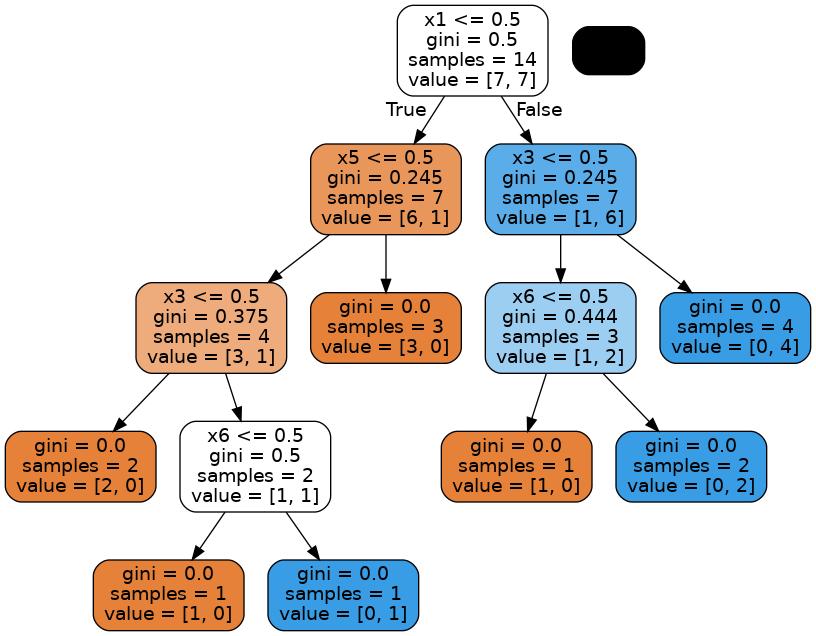
\includegraphics[width = 0.65\textwidth]{tree.png}
\end{figure}

Our code that utilizes the perceptron makes a perceptron makes a perceptron enacting the following linear equation:

\begin{equation}
    T = 8x_1 + 0x_2 + 4x_3 - x_4 -5 4x_5 + 3x_6 - 4
\end{equation}

\end{document}